\documentclass[tikz,border=5pt]{standalone}
\usepackage{tikz}
\usepackage{amsmath,amssymb}
\usetikzlibrary{arrows.meta,positioning,shapes.geometric,fit,backgrounds,calc,decorations.pathreplacing}

\definecolor{navy}{HTML}{1A365D}
\definecolor{accentblue}{HTML}{2B6CB0}
\definecolor{softblue}{HTML}{EBF8FF}
\definecolor{darkred}{HTML}{C53030}
\definecolor{softred}{HTML}{FFF5F5}
\definecolor{darkgreen}{HTML}{22543D}
\definecolor{softgreen}{HTML}{F0FFF4}
\definecolor{darkgold}{HTML}{975A16}
\definecolor{softgold}{HTML}{FEFCBF}
\definecolor{darkgray}{HTML}{2D3748}

\begin{document}
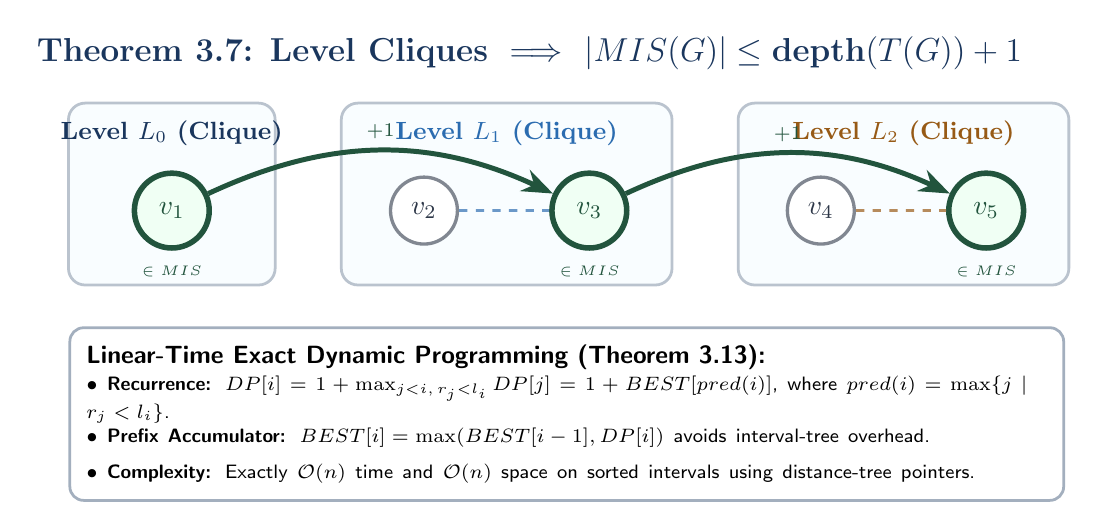
\begin{tikzpicture}[
    scale=1.05,
    >=Stealth,
    node distance=1.3cm,
    font=\sffamily,
    levelBox/.style={draw=navy!30, fill=softblue!30, rounded corners=6pt, line width=1pt},
    misNode/.style={circle, draw=darkgreen, fill=softgreen, line width=2pt, minimum size=0.95cm, inner sep=0pt, font=\bfseries, text=darkgreen},
    regNode/.style={circle, draw=darkgray!60, fill=white, line width=1.2pt, minimum size=0.85cm, inner sep=0pt, font=\bfseries, text=darkgray},
    dpEdge/.style={->, line width=1.8pt, draw=darkgreen}
]

    % ==========================================
    % LEVELS & INDEPENDENT SET BOUND
    % ==========================================
    \node[anchor=west, font=\bfseries\large, text=navy] at (0, 3.2) {\textbf{Theorem 3.7: Level Cliques $\implies$ $|MIS(G)| \le \text{depth}(T(G)) + 1$}};

    % Level 0 Box
    \draw[levelBox] (0.5, 0.4) rectangle (3.0, 2.6);
    \node[anchor=north, font=\bfseries\small, text=navy] at (1.75, 2.5) {Level $L_0$ (Clique)};
    \node[misNode] (u1) at (1.75, 1.3) {$v_1$};
    \node[below=2pt of u1, font=\tiny\bfseries, text=darkgreen] {$\in MIS$};

    % Level 1 Box
    \draw[levelBox] (3.8, 0.4) rectangle (7.8, 2.6);
    \node[anchor=north, font=\bfseries\small, text=accentblue] at (5.8, 2.5) {Level $L_1$ (Clique)};
    \node[regNode] (u2) at (4.8, 1.3) {$v_2$};
    \node[misNode] (u3) at (6.8, 1.3) {$v_3$};
    \draw[-, dashed, line width=1pt, draw=accentblue!70] (u2) -- (u3);
    \node[below=2pt of u3, font=\tiny\bfseries, text=darkgreen] {$\in MIS$};

    % Level 2 Box
    \draw[levelBox] (8.6, 0.4) rectangle (12.6, 2.6);
    \node[anchor=north, font=\bfseries\small, text=darkgold] at (10.6, 2.5) {Level $L_2$ (Clique)};
    \node[regNode] (u4) at (9.6, 1.3) {$v_4$};
    \node[misNode] (u5) at (11.6, 1.3) {$v_5$};
    \draw[-, dashed, line width=1pt, draw=darkgold!70] (u4) -- (u5);
    \node[below=2pt of u5, font=\tiny\bfseries, text=darkgreen] {$\in MIS$};

    % DP transitions
    \draw[dpEdge] (u1) to[bend left=25] node[midway, above, font=\scriptsize\bfseries, text=darkgreen] {$+1$} (u3);
    \draw[dpEdge] (u3) to[bend left=25] node[midway, above, font=\scriptsize\bfseries, text=darkgreen] {$+1$} (u5);

    % Callout Box Below
    \node[draw=navy!40, fill=white, rounded corners=5pt, line width=1pt, anchor=north west, inner sep=6pt, text width=12.2cm] at (0.5, -0.1) {
        \textbf{\small Linear-Time Exact Dynamic Programming (Theorem 3.13):}\\[2pt]
        \scriptsize
        $\bullet$ \textbf{Recurrence:} $DP[i] = 1 + \max_{j < i,\, r_j < l_i} DP[j] = 1 + BEST[pred(i)]$, where $pred(i) = \max \{j \mid r_j < l_i\}$.\\[1pt]
        $\bullet$ \textbf{Prefix Accumulator:} $BEST[i] = \max(BEST[i-1], DP[i])$ avoids interval-tree overhead.\\[1pt]
        $\bullet$ \textbf{Complexity:} Exactly $\mathcal{O}(n)$ time and $\mathcal{O}(n)$ space on sorted intervals using distance-tree pointers.
    };

\end{tikzpicture}
\end{document}
